\documentclass{beamer}
\usepackage{multicol}
\usepackage{xy}
\everymath{\displaystyle}
\mode<presentation>
{\usetheme{Warsaw}\setbeamercovered{dynamic}}
\usecolortheme{crane}
\usepackage{beamerfoils}
\pgfdeclareimage[height=1in]{university-logo}{ISULogo}
\logo{\pgfuseimage{university-logo}}
\setbeamertemplate{navigation symbols}{}
\title[\S8]{Section 8\\The Counting Principle and permutations}
\author{Dr Marcus Bishop}
\subject{Math 104}
\beamerdefaultoverlayspecification{<+->}
\theoremstyle{definition}
\newtheorem{remark}{Remark}
\newtheorem{impact}{Impact}
\newtheorem{notation}{Notation}
\newtheorem{question}{Question}
\usepackage{arev}
\begin{document}
\begin{frame}\titlepage\end{frame}
\LogoOff

\begin{frame}{Permutations}
\begin{itemize}
\item Ways of arranging set of distinct objects called
\alert{permutations}, \alert{arrangements}, or \alert{anagrams}
%\item Objects meant to be arranged linearly
\item Order matters in listing permutations
\item In contrast, order irrelevant in listing sets
\begin{example} Six permutations of $\left\{1,2,3\right\}$:
\[123\quad 132\quad 213\quad 231\quad 312\quad 321\]
\end{example}
\end{itemize}
\end{frame}

\begin{frame}
Permutations can be generated using tree diagram:
\[\begin{xy}<1.25cm,0cm>:
(0,0)="0";
(-3,-1)="-31";
(0,-1)="01";
(3,-1)="31";
"0";"-31"*+!D{1}**\dir{-};
"0";"01"*+!D{2}**\dir{-};
"0";"31"*+!D{3}**\dir{-};
"-31";(-4,-2)*+!D{2}**\dir{-};
(-4,-3)*+!D{3}**\dir{-};
"-31";(-2,-2)*+!D{3}**\dir{-};
(-2,-3)*+!D{2}**\dir{-};
"01";(-1,-2)*+!D{1}**\dir{-};
(-1,-3)*+!D{3}**\dir{-};
"01";(1,-2)*+!D{3}**\dir{-};
(1,-3)*+!D{1}**\dir{-};
"31";(2,-2)*+!D{1}**\dir{-};
(2,-3)*+!D{2}**\dir{-};
"31";(4,-2)*+!D{2}**\dir{-};
(4,-3)*+!D{1}**\dir{-};
\end{xy}\]
\end{frame}

\begin{frame}
\begin{itemize}
\item But drawing tree inefficient when only
\alert{number} of permutations needed
\item Observe that tree has $3$~branches,
each with $2$~branches, each with $1$~leaf
\item So $3\cdot 2\cdot 1=6$ leaves
\[\begin{xy}<1cm,0cm>:
(0,0)="0";
(-3,-1)="-31";
(0,-1)="01";
(3,-1)="31";
"0";"-31"*+!D{1}**\dir{-};
"0";"01"*+!D{2}**\dir{-};
"0";"31"*+!D{3}**\dir{-};
"-31";(-4,-2)*+!D{2}**\dir{-};
(-4,-3)*+!D{3}**\dir{-};
"-31";(-2,-2)*+!D{3}**\dir{-};
(-2,-3)*+!D{2}**\dir{-};
"01";(-1,-2)*+!D{1}**\dir{-};
(-1,-3)*+!D{3}**\dir{-};
"01";(1,-2)*+!D{3}**\dir{-};
(1,-3)*+!D{1}**\dir{-};
"31";(2,-2)*+!D{1}**\dir{-};
(2,-3)*+!D{2}**\dir{-};
"31";(4,-2)*+!D{2}**\dir{-};
(4,-3)*+!D{1}**\dir{-};
\end{xy}\]
\item Could use same mechanism to count permutations
of $\left\{1,2,3,4\right\}$ without drawing tree
\item Tree would have $4$~branches, each with $3$~branches,
each with $2$~branches, each with $1$~leaf
\item So tree would have $4\cdot 3\cdot 2\cdot 1=24$ leaves
\item So $24$ the number of permutations of four objects
\end{itemize}
\end{frame}

\begin{frame}{Factorial}
\begin{itemize}
\item Similarly $120=5\cdot 4\cdot 3\cdot 2\cdot 1$
the number of permutations of $5$ objects
\item In general $n\cdot\left(n-1\right)\cdot\left(n-2\right)
\cdots 3\cdot 2\cdot 1$ the number of permutations of $n$~objects
\item This number denoted by \alert{$n!$}
\item $n!$ pronounced \alert{$n$ factorial}
\item So $n!$ the number of permutations of $n$~objects
\end{itemize}
\end{frame}

\begin{frame}{Example from literature}
Murphy took the biscuits carefully out of the packet and laid them face
upward on the grass, in order as he felt of edibility. They were
the same as always, a Ginger, an Osborne, a Digestive, a Petit
Beurre and one anonymous. He always ate the first-named last, because
he liked it the best, and the anonymous first, because he thought
it very likely the least palatable. The order in which he ate the
remaining three was indifferent to him and varied irregularly from
day to day. On his knees now before the five it struck him for the
first time that this reduced to a paltry six the number of ways in
which he could make his meal.
\end{frame}
\begin{frame}
\dots Even if he conquered his
prejudice against the anonymous, still there would be only twenty-four
ways in which the biscuits could be eaten. But were he to take the
final step and overcome his infatuation with the ginger, then the
assortment would spring to life before him, dancing the radiant
measure of its total permutability, edible in a hundred and twenty
ways!\\
\hfill
from {\em Murphy} by Samuel Beckett
\end{frame}

\begin{frame}{Partial permutations}
\begin{itemize}
\item How many ways to arrange $6$ books on shelf?
\item $6!=6\cdot 5\cdot 4\cdot 3\cdot 2\cdot 1=720$
\item But what if shelf only has room for $3$ books?
\item Drawing tree cumbersome
\item If drawn, tree would have $6$~branches,
each with $5$~branches, each with $4$~leaves
\item Thus books can be arranged in $6\cdot 5\cdot 4=120$ ways
\item Slick way to write answer:
\[6\cdot 5\cdot 4
\only<+->{=\frac{6\cdot 5\cdot 4\cdot 3\cdot 2\cdot 1}
{3\cdot 2\cdot 1}}\only<+->{=\frac{6!}{3!}}
\only<+->{=\frac{6!}{\left(6-3\right)!}}\]
\item In general
$\frac{n!}{\left(n-r\right)!}$ the number of \alert{permutations
of $n$~objects taken $r$~at a time}
\item $\frac{n!}{\left(n-r\right)!}$ denoted
by \alert{$_nP_r$}
\end{itemize}
\end{frame}

\begin{frame}
\begin{example}
\begin{itemize}
\item Number of ways to arrange $6$~books
on shelf, taken from set of $10$~books:
\item $_{10}P_6
\only<+->{=\frac{10!}{\left(10-6\right)!}}
\only<+->{=\frac{10!}{4!}}
\only<+->{=10\cdot 9\cdot 8\cdot 7\cdot 6\cdot 5}
\only<+->{=151,200}$
\item Observe that $\frac{10!}{4!}$ faster to type
on calculator than 
$10\cdot 9\cdot 8\cdot 7\cdot 6\cdot 5$, if calculator
has \alert{$!$} button
\end{itemize}
\end{example}
\begin{example}
\begin{itemize}
\item Number of ways to select president, vice president,
and treasurer from among Alex, Brooke, Colby, and Denise:
\item $_4P_3
\only<+->{=\frac{4!}{\left(4-3\right)!}}
\only<+->{=4\cdot 3\cdot 2}
\only<+->{=24}$
\end{itemize}
\end{example}
\end{frame}

\begin{frame}{Counting principle}
\begin{itemize}
\item In general, to count ways task can be performed
\begin{itemize}
\item Organize task into stages
\item At each stage, a single decision should be made
\item Calculate number of ways decision can
be made at each stage
\item Multiply numbers
\end{itemize}
\item Division of task into ``stages'' sometimes unnatural,
artificial in context of problem
\begin{example}
\begin{itemize}
\item Consider example with Alex, Brooke, Colby, and Denise
\item First stage: select president
\item Can be done in $4$ ways
\item Second stage: select vice president
\item Can be done in $3$ ways, since one person already
chosen for president at this stage, etc.
\end{itemize}
\end{example}
\end{itemize}
\end{frame}

\begin{frame}{ATM PINs}
\begin{itemize}
\item An Automated Teller Machine (ATM)
allows bank customers to withdraw money from accounts
\item Customer must enter secret $4$-digit
Personal Identification Number (PIN)
\item Inventor John Shephard-Barron of ATM envisioned $6$-digit PINs
\item However, his wife preferred $4$-digit PINs
\begin{example}
\begin{itemize}
\item How many $4$-digit PINs possible?
\item First stage: choose first digit, \only<+->{can be done in $10$ ways}
\item Second stage: choose second digit, \only<+->{can be done in $10$ ways}
\item Similarly for third and fourth digits
\item So $10\cdot 10\cdot 10\cdot 10\only<+->{=10^4}$
\only<+->{$=10,000$ PINs possible}
\end{itemize}
\end{example}
\end{itemize}
\end{frame}

\begin{frame}{Iowa license plates}
\begin{multicols}{2}
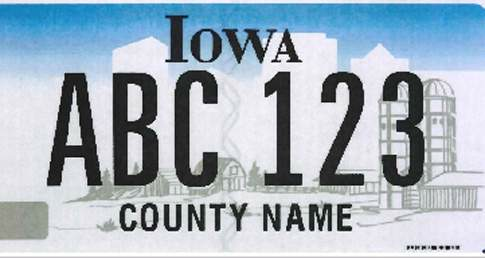
\includegraphics[scale=.3]{LicencePlate}
\begin{itemize}
\item Iowa license plates have three letters
and three digits
\item How many possible?
\item $26$ choices for first letter
\columnbreak
\item $26$ choices for second and third letters
\item $10$ choices for each of three digits
\item Thus $26\cdot 26\cdot 26\cdot 10\cdot 10\cdot 10$
\only<+->{$17,576,000$ plates possible}
\item Exceeds population of Iowa $\approx 3,000,000$
\end{itemize}
\end{multicols}
\end{frame}

\begin{frame}{Iowa area codes}
\begin{multicols}{2}
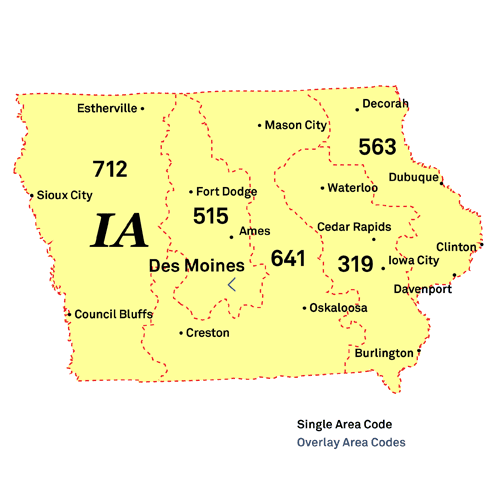
\includegraphics[scale=.35]{Iowa}
\begin{itemize}
\item Before 2000 Iowa had area codes $712$, $515$, and $319$
\item In 2000 Iowa introduced $641$ and $563$ due to increased usage
\item How many phone numbers within an area code?
\end{itemize}
\end{multicols}
\end{frame}

\begin{frame}{Phone numbers}
\begin{itemize}
\item Under North American Numbering Plan (NANP)
phone numbers consist of 
\begin{itemize}
\item three digit \alert{area code}
\item three digit \alert{exchange code}
\item four digit \alert{station code} or \alert{subscriber number}
\end{itemize}
\item First digit of exchange code can be $2$--$9$
\item $0$ reserved for calls to operator and 
$1$ reserved for signaling long-distance calls
\item All digits of station code and remaining digits
of exchange code can be $0$--$9$
\item Thus $8\cdot 10\cdot 10=800$ choices
for exchange code and $10\cdot 10\cdot 10\cdot 10=10000$
choices for station code
\item So $8,000,000$ numbers possible within area code
\end{itemize}
\end{frame}

\begin{frame}
\begin{itemize}
\item However, exchange codes of the form $X11$
reserved for municipal services, where $X$ one of $2$--$9$
\item So each of $211,311,\ldots,911$ eliminates $10,000$ phone numbers
\item So subtract $80,000$
\item Also, numbers 555-0100 through 555-0199 reserved for fiction
\item So subtract $100$
\item Thus $8,000,000-80,000-100=7,919,900$ phone numbers within an area code
\end{itemize}
\end{frame}

\begin{frame}{Anagrams}
\begin{itemize}
\item Anagrams of word \alert{bird}:
\begin{tabular}{cccccc}
bdir &bdri &bidr &bird &brdi &brid\\
dbir &dbri &dibr &dirb &drbi &drib\\
ibdr &ibrd &idbr &idrb &irbd &irdb\\
rbdi &rbid &rdbi &rdib &ribd &ridb 
\end{tabular}
\item Anagrams of word \alert{moon}:
\begin{tabular}{cccccc}
mnoo &mono &moon &nmoo &nomo &noom\\
omno &omon &onmo &onom &oomn &oonm 
\end{tabular}
\item Why more anagrams of \alert{bird} than \alert{moon}?
\item $24=4!$ the number of arrangements of four \alert{distinct} objects
\item But letters of \alert{moon} not distinct!
\item Hot to calculate number of anagrams?
\item Could try to list them, but listing highly error-prone
\end{itemize}
\end{frame}

%\begin{frame}{Rounding to three decimal places}
%\begin{itemize}
%\item All answer choices on quiz rounded to \alert{three} decimal places
%\item How to round to three decimal places:
%\begin{itemize}
%\item Write down three digits to right of decimal
%\item If $0$--$4$ the fourth digit then done
%\item However, if $5$--$9$ the fourth digit, then increase
%third digit by $1$
%\item \dots unless $9$ the third digit;
%\item \dots then increase \alert{second}
%digit by one and erase third digit
%\item Et cetera.
%\end{itemize}
%\item Answers \alert{unique} provided that everyone agrees
%to record answers in this format
%\end{itemize}
%\begin{example}
%\begin{itemize}
%\item Suppose $3.14159265358979$ the answer to question
%\item Then write $3.142$
%\end{itemize}
%\end{example}
%\end{frame}

\begin{frame}{Anagrams}
\begin{itemize}
\item To distinguish o's, color one red
\item Anagrams of word mo\alert{o}n:
\begin{tabular}{cccccc}
mno\alert{o}&mn\alert{o}o&mon\alert{o}&mo\alert{o}n\\
m\alert{o}no&m\alert{o}on&nmo\alert{o}&nm\alert{o}o\\
nom\alert{o}&no\alert{o}m&n\alert{o}mo&n\alert{o}om\\
omn\alert{o}&om\alert{o}n&onm\alert{o}&on\alert{o}m\\
o\alert{o}mn&o\alert{o}nm&\alert{o}mno&\alert{o}mon\\
\alert{o}nmo&\alert{o}nom&\alert{o}omn&\alert{o}onm
\end{tabular}
\item Anagrams of word moon:
\begin{tabular}{cccccc}
mnoo &mono &moon &nmoo &nomo &noom\\
omno &omon &onmo &onom &oomn &oonm 
\end{tabular}
\item Observe that each anagram of moon
appears \alert{twice} in list of anagrams of mo\alert{o}n 
\end{itemize}
\end{frame}

\begin{frame}
\begin{itemize}
\item But why twice?
\item Because $2=2!$ the number of ways to color o's
\begin{example} mono appears as anagram of mo\alert{o}n
as mon\alert{o} and m\alert{o}no
\end{example}
\item Thus number $N$ of anagrams of moon satisfies
\[24=2N\]
since $24=4!$ anagrams of mo\alert{o}n arise as colorings of
anagrams of moon
\item So $N=\frac{24}{2}=12$
\end{itemize}
\end{frame}

\begin{frame}
\begin{itemize}
\item Anagrams of epee (sword used in fencing):\\
\begin{tabular}{cccccc}
peee&epee&eepe&eeep
\end{tabular}
\item Anagrams of ep{\color{red}e}{\color{blue}e}:\\
\begin{tabular}{cccccc}
pe{\color{red}e}{\color{blue}e}&pe{\color{blue}e}{\color{red}e}&p{\color{red}e}e{\color{blue}e}&p{\color{red}e}{\color{blue}e}e\\
p{\color{blue}e}e{\color{red}e}&p{\color{blue}e}{\color{red}e}e&ep{\color{red}e}{\color{blue}e}&ep{\color{blue}e}{\color{red}e}\\
e{\color{red}e}p{\color{blue}e}&e{\color{red}e}{\color{blue}e}p&e{\color{blue}e}p{\color{red}e}&e{\color{blue}e}{\color{red}e}p\\
{\color{red}e}pe{\color{blue}e}&{\color{red}e}p{\color{blue}e}e&{\color{red}e}ep{\color{blue}e}&{\color{red}e}e{\color{blue}e}p\\
{\color{red}e}{\color{blue}e}pe&{\color{red}e}{\color{blue}e}ep&{\color{blue}e}pe{\color{red}e}&{\color{blue}e}p{\color{red}e}e\\
{\color{blue}e}ep{\color{red}e}&{\color{blue}e}e{\color{red}e}p&{\color{blue}e}{\color{red}e}pe&{\color{blue}e}{\color{red}e}ep
\end{tabular}
\item Each anagram of epee appears as anagram of
ep{\color{red}e}{\color{blue}e}
\alert{six} times
\item Why six?
\item Because $6=3!$ the number of ways to color the three e's
\item Thus number $N$ of anagrams of epee satisfies $24=6N$
\item So $N=\frac{24}{6}=4$
\end{itemize}
\end{frame}

\begin{frame}{Anagrams of kayak}
\begin{itemize}
\item Observe that $120=5!$ 
the number of anagrams of kay\alert{a}\alert{k} (not shown)
\item First four:
\begin{tabular}{cccc}
a\alert{a}k\alert{k}y
a\alert{a}\alert{k}ky
\alert{a}ak\alert{k}y
\alert{a}a\alert{k}ky
\end{tabular}
\item $2=2!$ ways to color a's
\item $2=2!$ ways to color k's
\item So $4=2!2!$ ways to color anagram
\item Thus number $N$ of anagrams satisfies
$120=4N$
\item So $N=\frac{120}{4}=30$
\end{itemize}
\end{frame}

\begin{frame}{General rule for number of anagrams}
\begin{itemize}
\item Suppose word has $n$ letters
\item But only $r$ letters $a_1,a_2,\ldots,a_r$ distinct 
\item Let $n_1$ be number of $a_1$'s
\item Let $n_2$ be number of $a_2$'s
\item $\vdots$
\item Let $n_r$ be number of $a_r$'s
\item Then $\frac{n!}{n_1!n_2!\cdots n_r!}$
the number of anagrams of word
\end{itemize}
\end{frame}

\begin{frame}{Example}
\begin{itemize}
\item Anagrams of \alert{plenipotentiary}
\item Count number of times each distinct letter appears:
\begin{tabular}{c|cccccccccc}
Letter&a&e&i&l&o&n&p&r&t&y\\\hline
Frequency&1&2&2&1&1&2&2&1&2&1
\end{tabular}
\item Confirm that word has $15$ letters and
$15=1+2+2+1+1+2+2+1+2+1$
\item Then number of anagrams
\[\frac{15!}{1!2!2!1!1!2!2!1!2!1!}
\only<+->{=\frac{15!}{2^5}}
\only<+->{=40,864,824,000}\]
\end{itemize}
\end{frame}

\begin{frame}{More realistic examples}
\begin{question}
\begin{itemize}
\item In how many ways can $3$~sets of plates be stacked in cupboard?
\item First set has $3$ identical plates
\item Second set has $4$, and third has $5$
\end{itemize}
\end{question}
\begin{itemize}
\item $3+4+5=12$ plates altogether
\item Denote a plate from first set by $A$
\item Denote plates from second, third sets by $B$, $C$
\item Using this notation
$AAABBBBCCCCC$ and $ABABCCBCCACB$ two possible stacking,
listed from top to bottom
\item Question asks for anagrams of $AAABBBBCCCCC$
\item So $\frac{12!}{3!4!5!}=27,720$ stackings
\end{itemize}
\end{frame}

\begin{frame}
\begin{question}
\begin{itemize}
\item Bag contains $3$~red and $3$~black balls
\item Balls drawn one at time without replacement
\item $\bullet\bullet\alert{\bullet}\bullet\alert{\bullet}\alert{\bullet}$
and $\alert{\bullet}\bullet\alert{\bullet}\bullet\bullet\alert{\bullet}$
two possible outcomes
\item How many outcomes possible?
\end{itemize}
\end{question}
\begin{itemize}
\item Question the same as previous anagram problems,
but with 
$\bullet\bullet\alert{\bullet}\bullet\alert{\bullet}\alert{\bullet}$
instead of English word
\item So $\frac{6!}{3!3!}=20$ possible outcomes
\end{itemize}
\end{frame}

\begin{frame}{Car keys (Exercise 63)}
\begin{question}
\begin{itemize}
\item Manufacturer plans to produce $400,000$ of a particular
model of car
\item Keys have $5$~cuts, each of $5$~possible depths
\item If not enough unique keys possible, then they plan to assign
each key to same number of cars
\item What is probability that randomly selected key
opens randomly selected car?
\end{itemize}
\end{question}
\begin{itemize}
\item $5^5=3125$ keys possible, so not enough for each car to have unique key
\item So each key opens $\frac{400000}{3125}=128$ cars
\item So $\frac{128}{400000}=\frac{1}{3125}=0.00032$
the probability that particular
key opens randomly selected car
\end{itemize}
\end{frame}

\end{document}
